\begin{surferPage}{Квинтика с $15$ каспами (точками возврата)\\{\normalfont\footnotesize(англ. „cusp“ — „заострение“)\par}}

Эта поверхность $5$ порядка (поэтому и название – квинтика) обладает $15$ сингулярностями типа $A_2$ (названных каспами или точками возврата), эту квинтику и серию родственных поверхностей впервые описал Оливер Лабс в 2005 г. 

Очевидно, пять сингулярностей выглядят не так как десять других. Пять сингулярностей относятся к типу $A_2^{++}$, а оставшиеся – к типу $A_2^{+-}$:
     \vspace*{-0.3em}
    \begin{center}
      \begin{tabular}{c@{\qquad}c}
        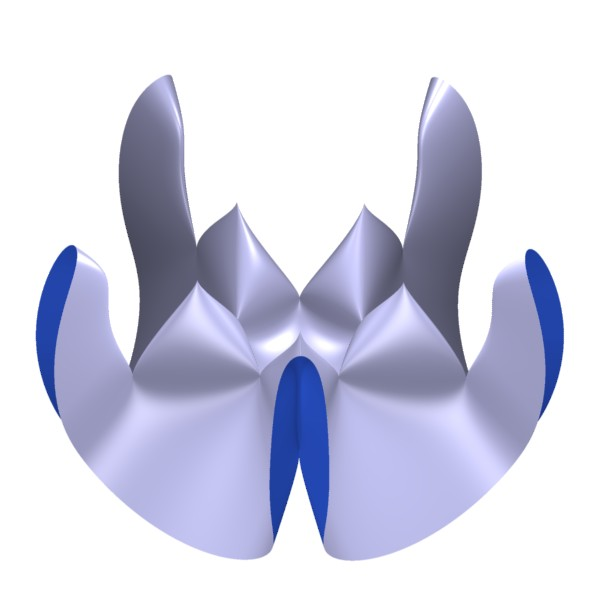
\includegraphics[height=1.2cm]{./../../common/images/dessins_quint_15a2}
        &
        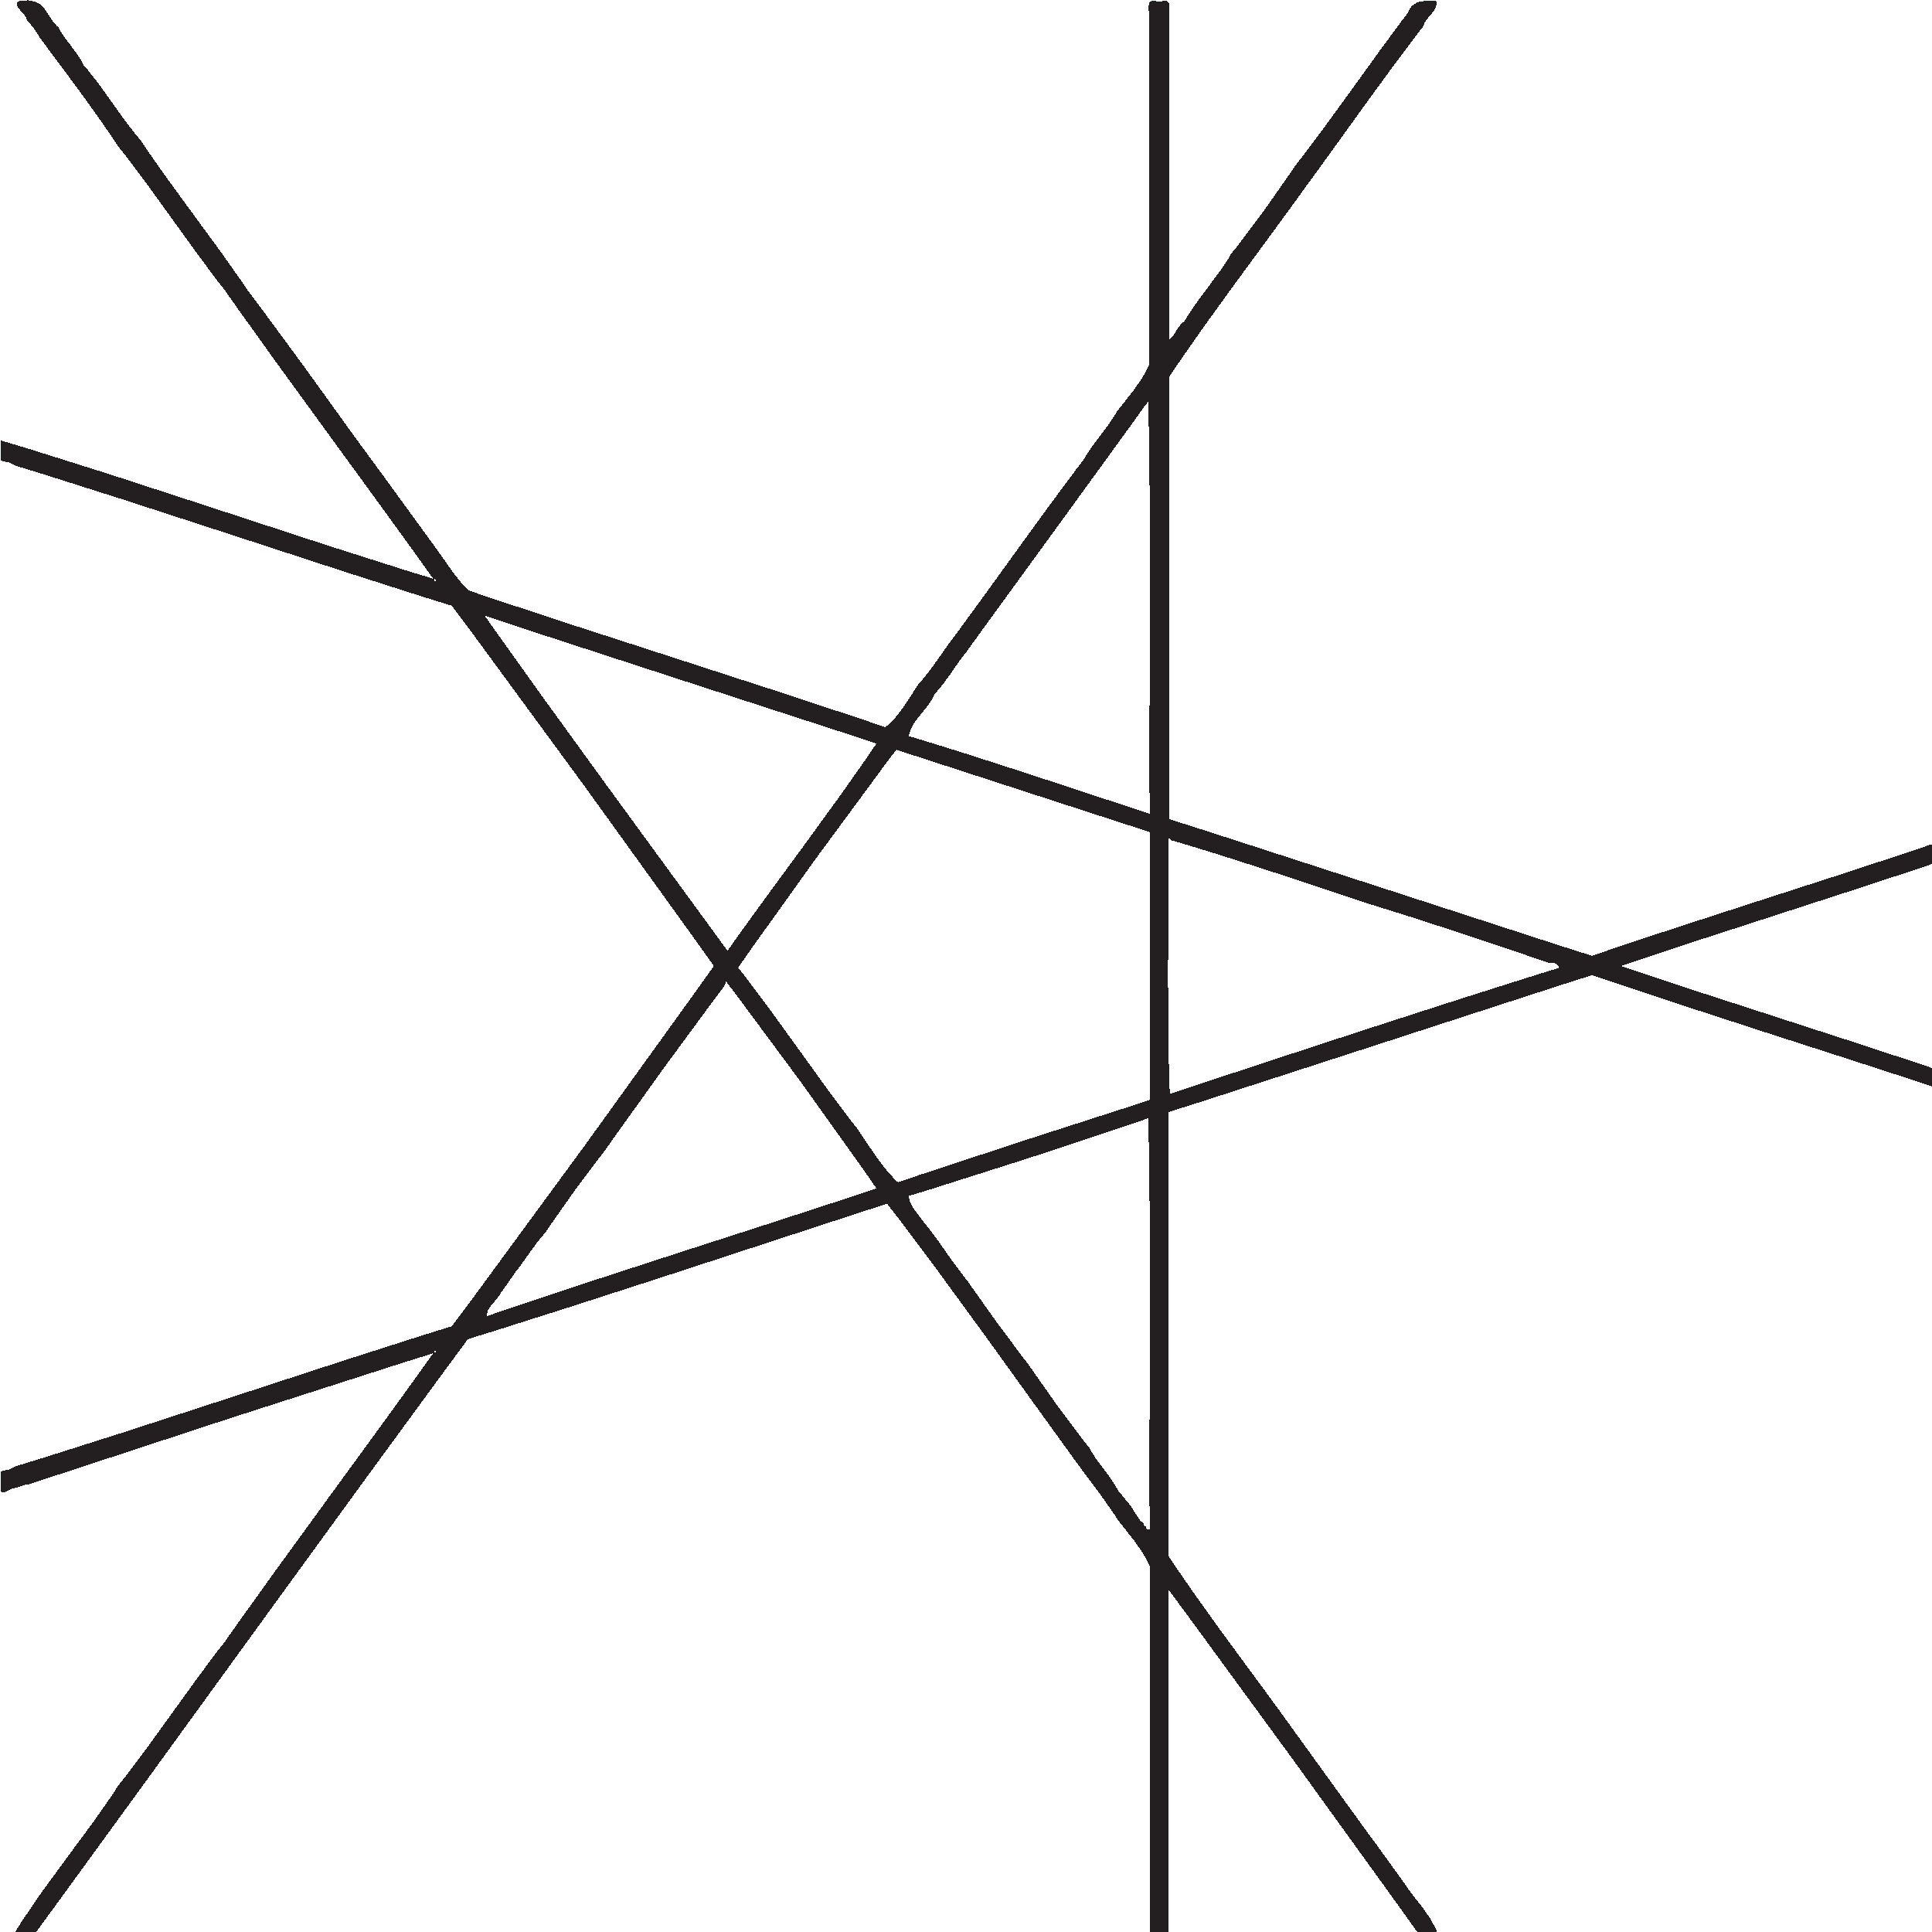
\includegraphics[height=1.2cm]{./../../common/images/rp5.pdf}
      \end{tabular}
    \end{center}
    \vspace*{-0.3em}    
    
    Эта поверхность имеет уравнение следующего вида:
    $S_5(x,y) + t(z)=0,$
    где $S_5(x,y)$ описывает правильный пятиугольник (изображение справа), а $t(z)$ - один из вариантов уже упоминавшихся многочленов Чебышёва.

Другая квинтика (слева) с $15$ каспами (точками возрата) описана Вольфом Бартом, она родственна кубике Клебша (справа). Обе они изображены на средней картинке:

    \vspace*{-1em}
    \begin{center}
      \begin{tabular}{c@{\quad}c@{\quad}c}
        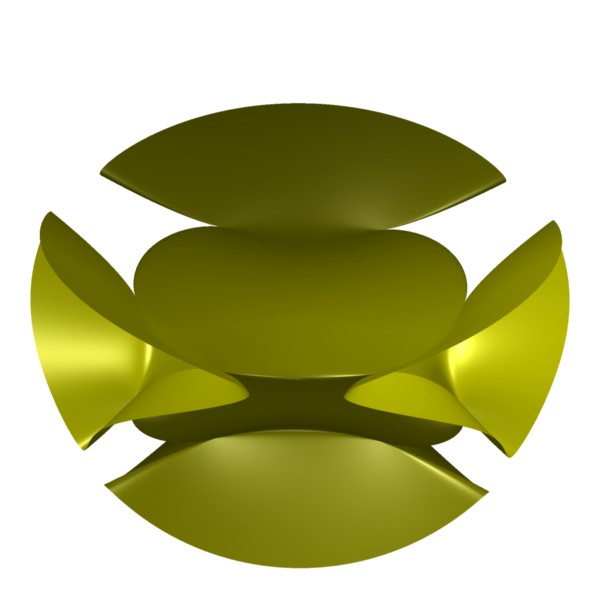
\includegraphics[height=1.2cm]{./../../common/images/barthquintic_green}
        &
        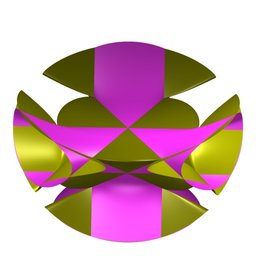
\includegraphics[height=1.2cm]{./../../common/images/barthquintic_clebschcubic}
        &
        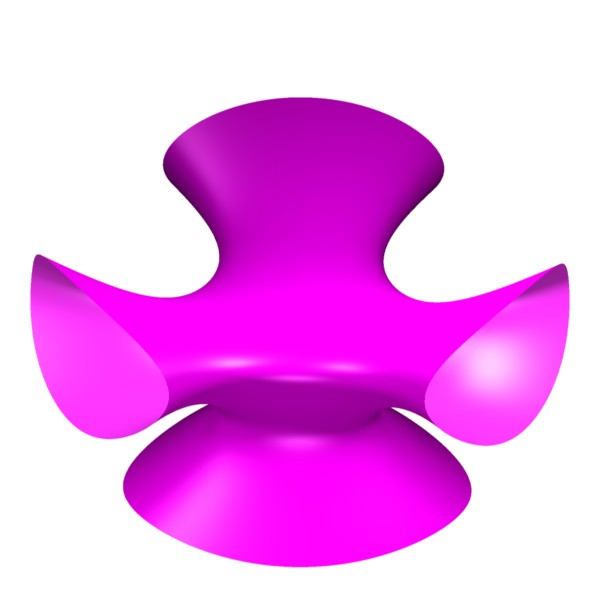
\includegraphics[height=1.2cm]{./../../common/images/clebschcubic_pink}
      \end{tabular}
    \end{center}
\end{surferPage}
